\documentclass[a4 paper, 11pt]{article}

\usepackage[top = 1.in, bottom = 1.in, left=0.7in, right = 0.7in]{geometry}

% fix figure positioning
\usepackage{float}

% tables
\renewcommand{\arraystretch}{1.4}
\usepackage{multirow}

% indent
\setlength{\parindent}{0em}

\usepackage{graphicx}
\usepackage{wrapfig}
%\begin{wrapfigure}{r}{2in}
%\centering
 %\includegraphics[width= 2.2in]{name of Image}
  %\caption {}
%\end{wrapfigure}
\usepackage{float}
\usepackage[ngerman]{babel}

\usepackage[hang]{footmisc}
\usepackage{multicol}
\usepackage[font={small,it}]{caption}

\usepackage{enumitem} 
%Liste Punkte (\begin {itemize}, \item)

%\usepackage{longtable} % Für Tabellen über 1 Seite
%\begin{longtable}{}
% \end{longtable}

\usepackage {setspace} %Zeilenabstand
%\begin{spacing}{Zahl}
%\end{spacing}

\usepackage{bm} %italic \bm{\mathit{•}}


\usepackage{siunitx}

\sisetup{locale = DE, per-mode = fraction, separate-uncertainty,   exponent-to-prefix, prefixes-as-symbols = false, scientific-notation=false
}
\newcommand{\ns}[4]{(\num[scientific-notation=false]{#1}\pm\num[scientific-notation=false]{#2})\cdot\num[]{e#3}\si{#4}}
% tables
\usepackage{multirow}

\begin{document}

\begin{titlepage}

\vspace*{1cm}
	\centering
	
	{\scshape\Large Protokolle Praktikum Physik 3cg \par}
	\vspace{0.5cm}
	{\huge\bfseries Experimentelle Bestimmung der spezifische Schmelzwärme von Eis\par}
	\vspace{0.5cm}
	{\Large Noah Vogt \& Simon Hammer\par}
	\vspace{0.5cm}

	{\large Durchgeführt am 15. September 2020\par}
	
\end{titlepage}

\tableofcontents
\pagebreak

\section{Versuchsziel}
Ziel ist es die \textit{spezifische Schmelzwärme} $L_f$ von Eis mittels eines\textit{kalorimetrischen Experiments} so genau wie möglich zu bestimmen und mit dem Tabellenwert $ \num{3.338 e5}\si{\J\per\kg} $ zu vergleichen und die abbweichung vom Tabellenwert zu erklären.

\section{Physikalischer Hintergrund}
Die Schmelzwärme ist die menge an Energie die aufgebracht werden muss, um den Aggregatzustand eines Stoffes von fest zu flüssig oder umgekehrt zu ändern, ohne das sich die Temperatur, bei konstantem Druck, verändert. Sie ist abhängig von der Masse und dem Stoff an sich. Die zur Schmelzwärme gehörende konstante ist die \textit{spezifische Schmelzwärme}, welche sich auf die Masse bezieht und die Einheit $\si{\J\per\kg}$ hat. Nach diesem Model lautet nun die Formel für die Schmelzwärme 
$$ Q_{schmelz}= m \cdot L_f$$
Bei einem \textit{kalorimetrischen Experiment} wird von einem idealisierten abgeschlossenen Systeme ausgegangen. Es wird angenommen, dass die vom Wasser abgegebene Wärme der vom Eis aufgenommenen Wärme entspricht. Spricht:
$$ Q_{Auf}=Q_{Ab}$$
Das Eis wird zwei physikalisch wichtige Prozesse durchgehen. Wir nehem an dass das Eis anfangs $\SI{0}{\celsius}$ hat. Zuerst wird das Eis geschmolzen und dann erwärmt. Daraus folgt das die Schmelzwärme zur Wärmemenge addiert werden muss, um die menge an Wärme zu erlangen welche gebraucht wird um das Eis zu schmelzen und auf eine bestimmte Temperatur zu erwärmen. (Für die vereinfachung nene wir die Schmelzwärme $Q_{1}$ und die benötigte Wärme um das geschmolzene Eis zu erwärmen $Q_{2}$, die abgegebene Wärme des heissen Wasser nenen wir $Q_{3}$). Die Formel lautet somit
$$ Q_{1} + Q_{2} = Q_{3} $$
Die Formel für die Wärmemenge wird aus der Formelsammlung entnommen.
$$ Q_{1} + Q_{2} = Q_{3} \Rightarrow m_{\rm{Eis}} \cdot L_f + m_{\rm{Eis}} \cdot c_{\rm{H_2O}} \cdot \mathit{\Delta}\vartheta_1 = m_{\rm{H_2o}} \cdot c_{\rm{H_2o}} \cdot \mathit{\Delta}\vartheta_2$$ $$ \Rightarrow L_f = \frac{m_{\rm{H2O}} \cdot c_{\rm{H_2o}} \cdot \mathit{\Delta}\vartheta_2 - m_{\rm{Eis}} \cdot c_{\rm{H_2O}} \cdot \mathit{\Delta}\vartheta_1}{m_{\rm{Eis}}}$$



\section{Versuchsaufbau}
\begin{figure}[H]
    \centering
    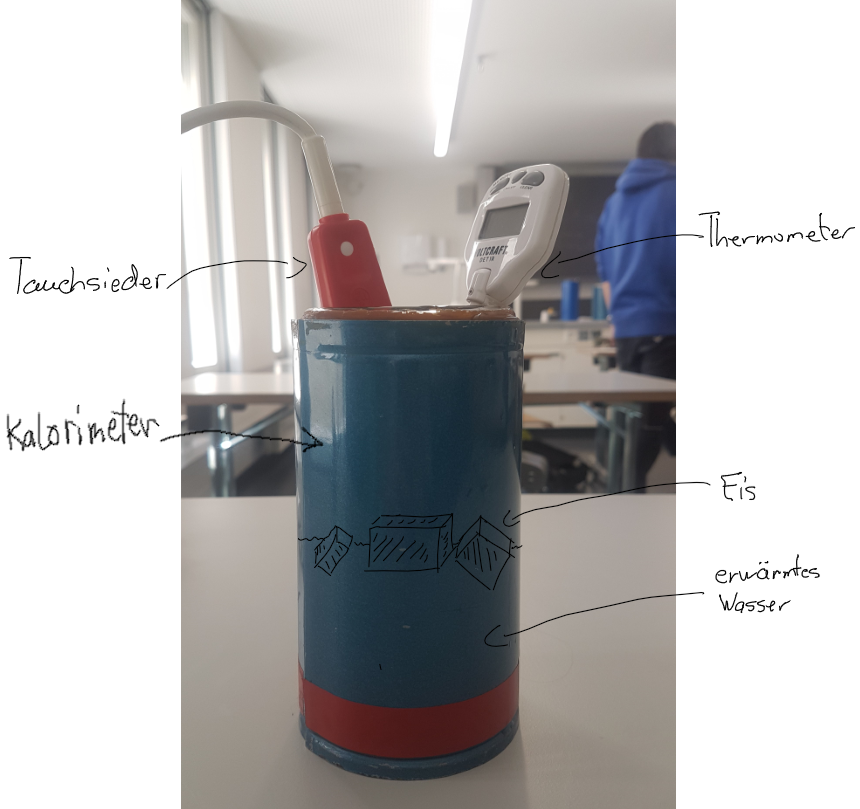
\includegraphics[width=.5\linewidth]{image}
\end{figure}

\section{Versuchsdurchführung}
\begin{table}[H]
    \centering
    \begin{tabular}{|c|c|c|}
        \hline
        \textbf{Beschreibung} & \textbf{Abkürzung} & \textbf{Wert} \\
        \hline
        Wärmekapazität Wasser & $C_{H_{2}O}$ & 4182 $\frac{J}{kg\cdot{}K}$\\
        \hline
        Masse Kalorimeter leer & $m_{Kal}$ & $(613.0\pm 0.05)g$\\
        Masse Kalorimeter mit Wasser 1 & $m_{1}$ & $(787.0\pm 0.05)g$\\
        \hline
        Masse Gemischt 1 & $m_{2}$ & $(796.9\pm 0.05)g$\\
        Masse Kalorimeter mit Wasser 2 & $m_{3}$ & $(781.3\pm 0.05)g$\\
    Masse Gemischt 2 & $m_{4}$ & $(795.8\pm 0.05)g$\\
        \hline
        Temperatur vor dem Eis 1 & $\vartheta_{T_{1}}$ & $(70.3\pm 0.05)^{\circ}C$\\
        Temperatur geschmolzen 1 & $\vartheta_{T_{2}}$ & $(62.7\pm 0.05) ^{\circ}C$\\
        \hline
        Temperatur vor dem Eis 2 & $\vartheta_{T_{3}}$ & $(63.4\pm 0.05)^{\circ}C$\\
        Temperatur geschmolzen 2 & $\vartheta_{T_{4}}$ & $(54.1\pm 0.05) ^{\circ}C$\\
        \hline
    \end{tabular}
\end{table}
Als erstes wird die Masse des Kalorimeters $m_{\rm{Kal}} $ gemessen  und bis zur hälfte etwa mit Wasser gefühlt. Die Masse des Kalorimeters mit dem Wasser $m_{\rm{1/3}} $ wird nun nochmal gemessen. Das sich im Kalorimeter befindende Wasser wird nun, mit dem Tauchsieder, auf etwa   $\SI{70}{\celsius} $ erwärmt. Das Eis wird abgetrocknet und die Teperatur des heissen Wassers $\vartheta_{T_{1/3}} $ bis kurz vor dem hinzugeben des Eises abgelesen. 
\section{Versuchsauswertung}

\subsection{Durchführung 1}

$L_{f_1}= \displaystyle{\frac{m_{\rm{H2O}} \cdot c_{\rm{H_2o}} \cdot \mathit{\Delta}\vartheta_2 - m_{\rm{Eis}} \cdot c_{\rm{H_2O}} \cdot \mathit{\Delta}\vartheta_1}{m_{\rm{Eis}}}}$\\\\

$L_{f_1}=\displaystyle{\frac{\left(\left(m_1-m_{Kal}\right) \cdot 4182\frac{J}{Kg \cdot K}\cdot \Delta \vartheta_{T_1}\right)-\left(\left(m_2-m_{Kal}\right)\cdot 4182 \frac{J}{Kg \cdot K} \cdot \vartheta_{T_2}\right)}{m_2-m_{Kal}}} $\\\\

$L_{1_{max}} =\displaystyle{\frac{\left(0.174Kg \cdot 4182\frac{J}{Kg \cdot K}\cdot \right)-\left(\left(m_2-m_{Kal}\right)\cdot 4182 \frac{J}{Kg \cdot K} \cdot \vartheta_{T_2}\right)}{m_2-m_{Kal}}} $

\subsection{Durchführung 2}
$L_{f_2} = \displaystyle{\frac{m_{\rm{H_{2}O}} \cdot c_{\rm{H_{2}O}} \cdot \Delta\vartheta_2 - m_{\rm{Eis}} \cdot c_{\rm{H_2O}} \cdot \Delta\vartheta_1}{m_{\rm{Eis}}}}$
\section{Kommentar / Diskussion}

Masse fehlerrechnung wurde vernachlässigt



\end{document}
